\documentclass[12pt,letterpaper]{article}
\usepackage[utf8]{inputenc}
\usepackage{amsmath,amsthm,amsfonts,amssymb,amscd}
\usepackage[table]{xcolor}
\usepackage[margin=4cm]{geometry}
\usepackage{ragged2e}
\usepackage{graphicx}
\usepackage{multicol}
\usepackage{csquotes}
\usepackage{listings}
\usepackage{float}
\usepackage[makeroom]{cancel}
\usepackage{color}
%\usepackage[brazil]{babel}

\newlength{\tabcont}
\setlength{\parindent}{0.3in}
\setlength{\parskip}{0.05in}

\definecolor{dkgreen}{rgb}{0,0.6,0}
\definecolor{gray}{rgb}{0.5,0.5,0.5}
\definecolor{mauve}{rgb}{0.58,0,0.82}

\lstset{frame=tb,
  language=C,
  aboveskip=3mm,
  belowskip=3mm,
  showstringspaces=false,
  columns=flexible,
  basicstyle={\small\ttfamily},
  numbers=none,
  numberstyle=\tiny\color{gray},
  keywordstyle=\color{blue},
  commentstyle=\color{dkgreen},
  stringstyle=\color{mauve},
  breaklines=true,
  breakatwhitespace=true,
  tabsize=2
}

\title{MAC0328 - Lista 2}
\author{Lucas Santos}
\date{Agosto 2017}

\begin{document}

\maketitle

\textbf{Notação.} Definimos $a \sim b$ como um caminho saindo de $a$ e indo para $b$. Adicionalmente, definimos $a \stackrel{s}{\sim} b$ como um caminho \textit{simples} saindo de $a$ e indo para $b$.

\section {Exercícios opcionais}

\begin{enumerate}
    \item Vamos começar provando a ida. Suponha um grafo $G$ que possui um caminho $k_1$ com origem $s$ e término $t$. Isto é,
    $$ k_1 = s \sim t$$
    Se $k_1$ for um caminho simples, então já está provado. Caso não seja, ele pode ser descrito como
    $$ k_1 = (s \sim w) \cup (w \sim w) \cup (w \sim t)$$
    para algum $w \in G_V$. Então basta tomar
    $$ k_2 = (s \sim w) \cup (w \sim t) $$
    Fazemos esse processo enquanto houverem ciclos no caminho. No final, mostramos que existe um caminho simples em $G$.

    A prova da volta é direta: basta ver que por definição um caminho simples é um caminho. Logo, dado um grafo $G$ e um caminho simples $k$ com origem $s$ e término $t$, então o caminho simples $k$ é, por definição, um caminho de $G$.

    \item Seja $G$ um grafo-caminho com $V$ vértices com $V-1$ arcos da forma 0-1, 1-2, ..., (V-2)-(V-1). A topologia identidade, isto é $topo[v] \equiv v$, é uma topologia possível para o grafo $G$ pois segue que
    $$ 0 < 1 < ... < V-2 < V-1 $$
    Logo, todo grafo-caminho é topológico.

    \item \textit{Assumindo uma estrutura de dados de listas de adjacência para representação do grafo.} O algoritmo apresenta complexidade de tempo $O(V+A)$ e de espaço constante.
    \begin{lstlisting}
        int GRAPHtopologic (Graph G, int *vv) {
            Vertex v;
            link p;
            for (v = 0; v < G->V; v++)
                for (p = G->adj[v]; p != NULL; p = p->next)
                    if (vv[v] >= vv[p->w])
                        return 0;
            return 1;
        }
    \end{lstlisting}

    \item Seja $G$ um grafo topológico com $V$ vértices, $topo[]$ a numeração topológica do grafo $G$ e $V^*$ uma permutação de $V$ tal que
    $$ topo[V^*_1] < topo[V^*_2] < ... < topo[V^*_{|V|}] $$
    Observe que $V^*_1$ pode ser a origem de qualquer arco com término em $V^*_i$ com $1 < i \leq |V|$. Analogamente, para o vértice $V^*_j$, $j \in V$, $V^*_j$ pode ser a origem de qualquer arco com término em $V^*_i$ com $j < i \leq |V|$.
    A soma do número máximo de arcos possíveis é dada, então, por
    $$ \sum_{i = 1}^{|V|} (|V| - i) = \sum_{i = 0}^{|V|-1} i = \frac{|V|(|V|-1)}{2} $$

    \item Sim, é verdade. Basta tomar
    $$ p[0] = 0, p[1] = 0, p[2] = 1, ..., p[V] = V-1$$

    \item A ideia do algoritmo abaixo é verificar, para todo vértice, qual a altura dele na sua árvore radicada. Então, pegamos a maior das alturas e, por tanto, profundidade de um vértice de profundidade máxima. O algoritmo apresenta complexidade de tempo $O(V^2)$ e complexidade de espaço constante.
    \clearpage
    \begin{lstlisting}
        int GRAPHrootedForestHeight (Graph G, int *p) {
            Vertex v, w;
            int alturaAtual;
            int alturaMaxima = 0;
            for (v = 0; v < G->V; v++) {
                w = v;
                alturaAtual = 0;
                while (w != p[w]) {
                    alturaAtual++;
                    w = p[w];
                }
                alturaMaxima = max (alturaMaxima, alturaAtual);
            }
            return alturaMaxima;
        }
    \end{lstlisting}

    \item Assumindo a existência da função $randV$ visto em aula (a função devolve um vértice $v \in V$ aleatório). Considerando a representação do grafo por matrizes de adjacência, temos uma complexidade de tempo igual a $O(V)$ e espaço constante.
    \begin{lstlisting}
        Graph GRAPHbuildRandRootedTree (int V) {
            Vertex v;
            Graph G = malloc (sizeof * G);
            Graph->V = V;
            Graph->A = V - 1;
            for (v = 0; v < G->V; v++)
                GRAPHinsertArc (G, randV (V), v);
            return G;

        }
    \end{lstlisting}

    \item A implementação iterativa pode ser feita utilizando uma pilha.
    \begin{lstlisting}
        int GRAPHreach (Graph G, Vertex s, Vertex t)
        {
            Vertex stack[G->V], w;
            int stackSize = 0;
            for (vertex v = 0; v < G->V; ++v)
                visit[v] = 0;
            stack[stackSize++] = v; // Adiciona o vertice inicial na pilha
            visit[v] = 1; // Marca o vertice inicial como visitado
            while (stackSize > 0) {
                w = stack[stackSize--];
                for (link a = G->adj[w]; a != NULL; a = a->next)
                    if (visit[a->w] == 0) {
                        stack[stackSize++] = a->w;
                        visit[a->w] = 1;
                        if (a->w == w)
                            return (1);
                    }
            }
            return (0);
        }
    \end{lstlisting}

    \item \textit{Assumindo a implementação recursiva do $reachR$ que para e retorna se encontrar o vértice alvo.}
    \begin{figure}[h]
    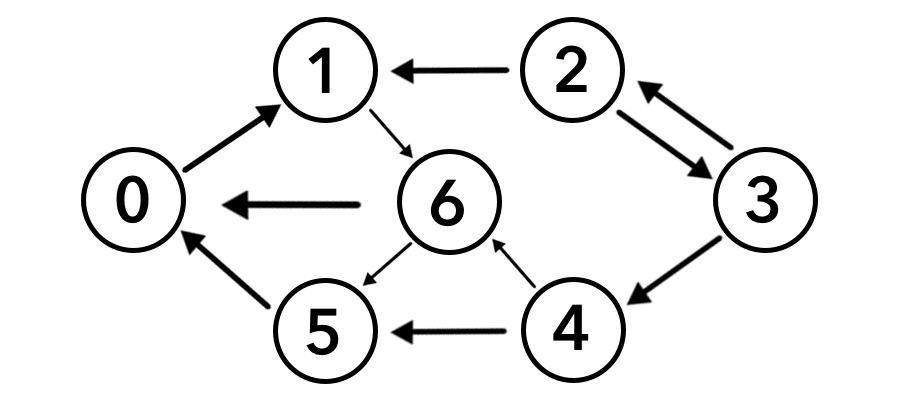
\includegraphics[width=8cm]{graph.png}
    \centering
    \end{figure}

    Note que os nós que não possuem arestas são descartados da forma \cancel{1} e nós já visitados são descartados da forma \bcancel{1}.

    Simulando a chamada $GRAPHreach(G, 3, 0)$:

    \fbox{\begin{minipage}{15em}
        Chamada $s = 3, t = 0$\\
        $w = \cancel{0} \; \cancel{1} \; 2$

        \fbox{\begin{minipage}{14.5em}
            Chamada $s = 2, t = 0$\\
            $w = \cancel{0} \; 1$

            \fbox{\begin{minipage}{14em}
                Chamada $s = 1, t = 0$\\
                $w = \cancel{0} \; \cancel{1} \; \cancel{2} \; \cancel{3} \; \cancel{4} \; \cancel{5} \; 6$

                \fbox{\begin{minipage}{13.5em}
                    Chamada $s = 6, t = 0$\\
                    $w = \cancel{0} \; \cancel{1} \; \cancel{2} \; \cancel{3} \; \cancel{4} \; 5

                    \fbox{\begin{minipage}{13em}
                        Chamada $s = 5, t = 0$\\
                        $w = 0$, logo retorna 1.
                    \end{minipage}}

                    Retorna 1.
                \end{minipage}}
                Retorna 1.
            \end{minipage}}
            Retorna 1.
        \end{minipage}}
        Retorna 1.
    \end{minipage}}

    Simulando a chamada $GRAPHreach(G, 0, 3)$:

    \fbox{\begin{minipage}{15em}
        Chamada $s = 0, t = 3$\\
        $w = \cancel{0} \; 1 \; \cancel{2} \; \cancel{3} \; \cancel{4} \; \cancel{5} \; \cancel{6}

        \fbox{\begin{minipage}{14.5em}
            Chamada $s = 1, t = 3$\\
            $w = \cancel{0} \; \cancel{1} \; \cancel{2} \; \cancel{3} \; \cancel{4} \; \cancel{5} \; 6

            \fbox{\begin{minipage}{14em}
                Chamada $s = 6, t = 3$\\
                $w = \bcancel{0} \; \cancel{1} \; \cancel{2} \; \cancel{3} \; \cancel{4} \; 5 \; \cancel{6}$

                \fbox{\begin{minipage}{13.5em}
                    Chamada $s = 5, t = 3$\\
                    $w = \bcancel{0} \; \cancel{1} \; \cancel{2} \; \cancel{3} \; \cancel{4} \; \cancel{5} \; \cancel{6}$ \\
                    Retorna 0.
                \end{minipage}}
                Retorna 0.
            \end{minipage}}
            Retorna 0.
        \end{minipage}}
        Retorna 0.
    \end{minipage}}
\end{enumerate}

\section {Relatório do exercício 10}

\subsection {Introdução}
Dado um grafo $G$ não digirido com $V$ vértices e número esperado de arestas $E$, podemos inferir uma probabilidade $p_e$ de uma aresta estar presente no grafo $G$.
Como temos a restrição de termos um número esperado $E$ de arestas, definimos a probabilidade $p_e$ como
$$ p_e = \frac{E}{E_{max}} = \frac{2E}{V * (V-1)} $$
onde
$$ E_{max} = \frac{V * (V-1)}{2} $$

É interessante perceber que isso define um grafo randômico no modelo Erdős–Rényi. Iremos analisar esse tópico após os experimentos.

O problema consiste em determinar experimentalmente a probabilidade $p$ de dois vértices escolhidos aleatoriamente estejam ao alcance um do outro, isto é, dados dois vértices $u, v$ aleatórios, verificar a probilidade de existir um caminho $u \sim v$.

\subsection {Experimentos}
Para os experimentos, iremos usar $V = \{ 10, 50, 100, 1000, 10000 \}$. Para cada $v \in V$, iremos variar $E$ no intervalo $[0, E_{max}]$ ou até que $p = 1$.
Por fim, para cada configuração $G(V, E)$, iremos a usar a estrutura de dados de conjuntos disjuntos (\textit{Union-Find}) para computar a alcançabilidade de todo par de vértices (se dois vértices estão no mesmo conjunto, então são alcançaveis entre si).

A probabilidade $p$ é definida então como
$$ p = \frac{\text{pares de vértices com caminho entre si}}{\text{todos os pares de vértices}} $$

Finalmente, estamos interessados em alguns aspectos:
\begin{enumerate}
    \item O valor de $E$ que torna a probabilidade $p = 1$;
    \item Número de componentes por configuração;
\end{enumerate}

\textit{Os códigos utilizados para gerar os experimentos abaixo estão em anexo. As imagens foram geradas usando ferramentas auxiliares (Google Sheets).}

Quanto à probabilidade, temos os seguintes resultados.

\begin{figure}[H]
    \subfigure{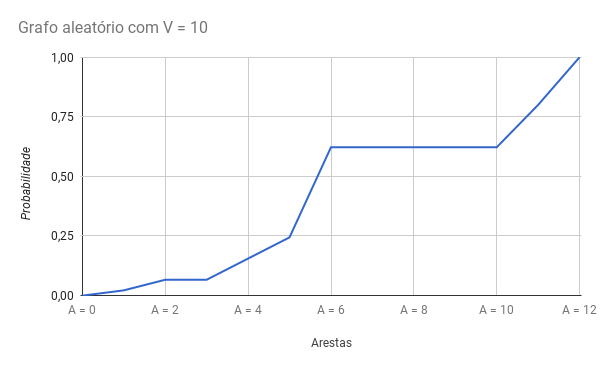
\includegraphics[width=7cm]{chart-10.png}}
    \subfigure{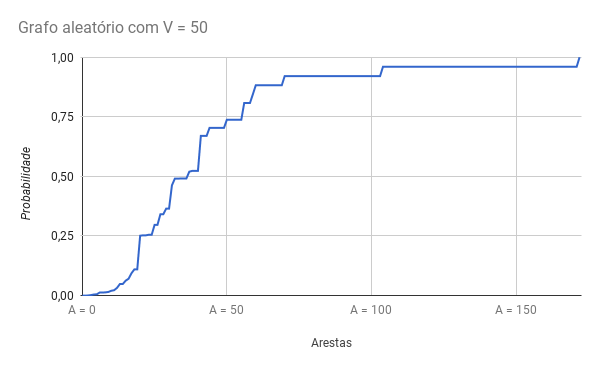
\includegraphics[width=7cm]{chart-50.png}}
\end{figure}

\begin{figure}[H]
    \subfigure{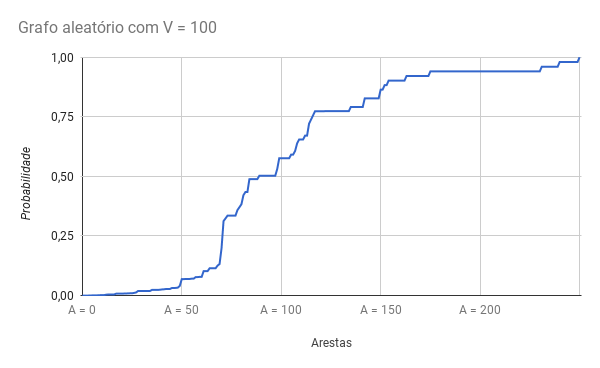
\includegraphics[width=7cm]{chart-100.png}}
    \subfigure{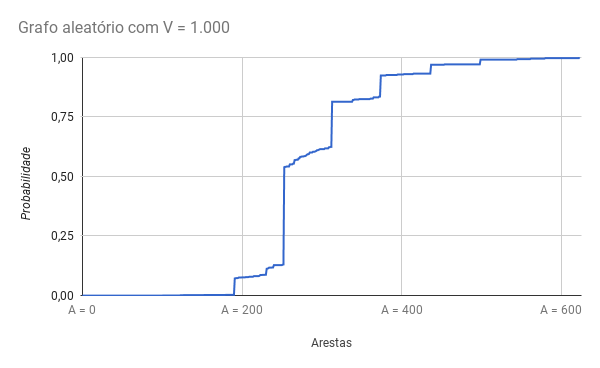
\includegraphics[width=7cm]{chart-1000.png}}
\end{figure}

\begin{figure}[H]
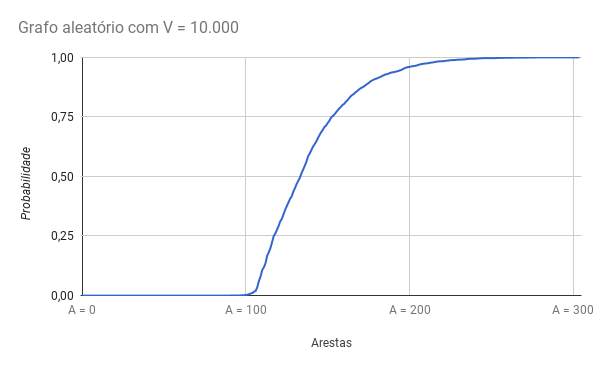
\includegraphics[width=7cm]{chart-10000.png}
\centering
\end{figure}

Quanto ao número de componentes, temos os seguires resultados.

\begin{figure}[H]
    \subfigure{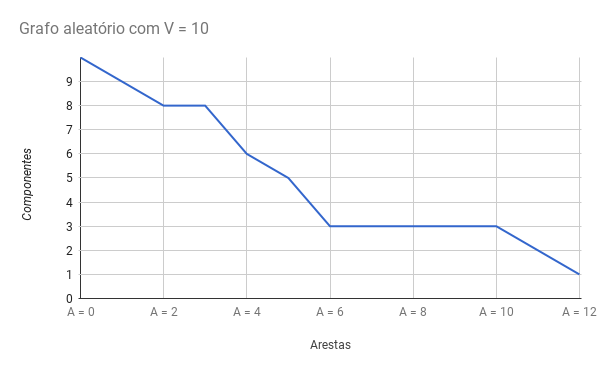
\includegraphics[width=7cm]{comp-10.png}}
    \subfigure{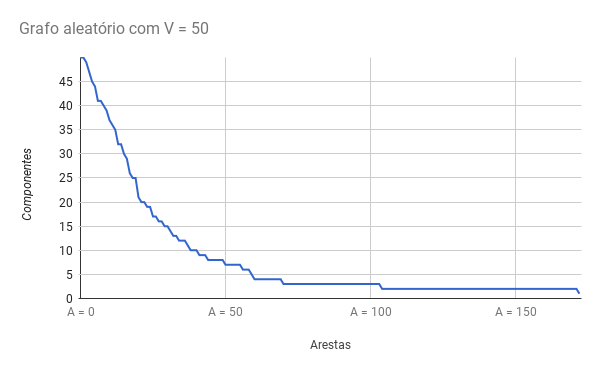
\includegraphics[width=7cm]{comp-50.png}}
\end{figure}

\begin{figure}[H]
    \subfigure{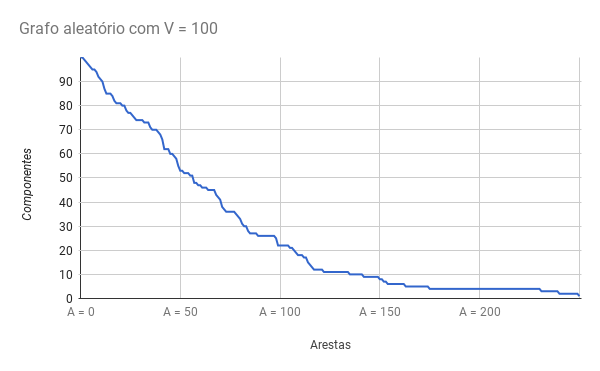
\includegraphics[width=7cm]{comp-100.png}}
    \subfigure{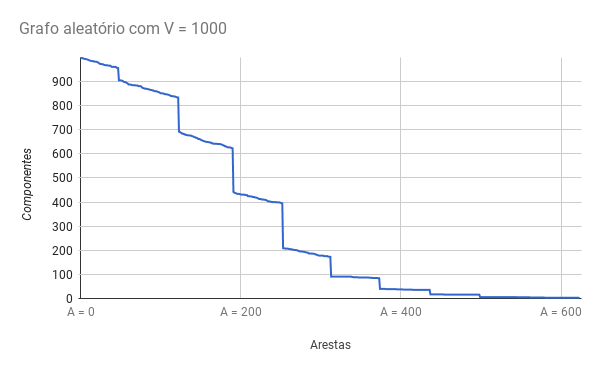
\includegraphics[width=7cm]{comp-1000.png}}
\end{figure}

\begin{figure}[H]
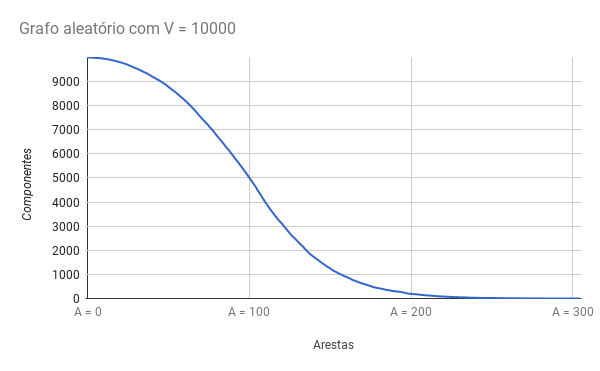
\includegraphics[width=7cm]{comp-10000.png}
\centering
\end{figure}

\subsection {Mais sobre o modelo Erdős–Rényi}
O modelo Erdős–Rényi apresenta algumas propriedades interessantes e, entre elas, uma que diz

\enquote{Quase todos os grafos com $p_e = \frac{2*ln(V)}{V}$ são conectados.}\footnote{https://en.wikipedia.org/wiki/Erdős–Rényi_model}

Fazendo os cálculos inversos para obter os valores de $E$ tal que $p_e = \frac{2*ln(V)}{V}$ para cada $v \in V$, temos:
$$ p_e = \frac{E}{E_{max}} = \frac{2E}{V * (V-1)} $$
$$ p_e = \frac{2*ln(V)}{V} $$
$$ E = p_e * V * (V - 1) = 2 * ln(V) * (V - 1) $$

Agora para cada $v \in V$:
\begin{enumerate}
    \item $v = 10$, temos que $E \approx 41$ (alcançamos $p = 1$ com $E \approx 12$);
    \item $v = 50$, temos que $E \approx 383$ (alcançamos $p = 1$ com $E \approx 172$);
    \item $v = 100$, temos que $E \approx 911$ (alcançamos $p = 1$ com $E \approx 250$);
    \item $v = 1.000$, temos que $E \approx 13.801$ (alcançamos $p = 1$ com $E \approx 623$);
    \item $v = 10.000$, temos que $E \approx 184.188$ (alcançamos $p = 1$ com $E \approx 304$);
\end{enumerate}

Experimentalmente, pudemos verificar que de fato $p_e = \frac{2*ln(V)}{V}$ é de fato um bom limite inferior.

\subsection {Conclusão}
Pudemos verificar que conforme o número de arestas cresce, maior a probabilidade do grafo estar conectado e, portanto, maior a probabilidade de dois vértices aleatórios estarem ao alcance um do outro.

Foi interessante verificar que existe um modelo, o de Erdős–Rényi, que descreve tal grafo aleatório e, mais que isso, verificar seu funcionamento experimentalmente.

Para trabalhos futuros, talvez seja interessante entender como grafos esparsos se comportam com esse modelo uma vez que por limitação de tempo e processamento, foram escolhidos pequenas quantidades de vértices. Tal escolha pode ter levado esse experimento a algum viés não observado.

\end{document}
